\documentclass{article}

\usepackage{graphicx}
\usepackage{tikz}
\usepackage{tikzsymbols}
\usetikzlibrary{calc,patterns,shapes.geometric}
\pagestyle{empty}
\usepackage[margin=0pt]{geometry}
\geometry{papersize={14in,12in}}

\def\centerarc[#1](#2)(#3:#4:#5){\draw[#1] ($(#2)+({#5*cos(#3)},{#5*sin(#3)})$) arc (#3:#4:#5);}

\begin{document}
	\begin{figure}
		\centering
		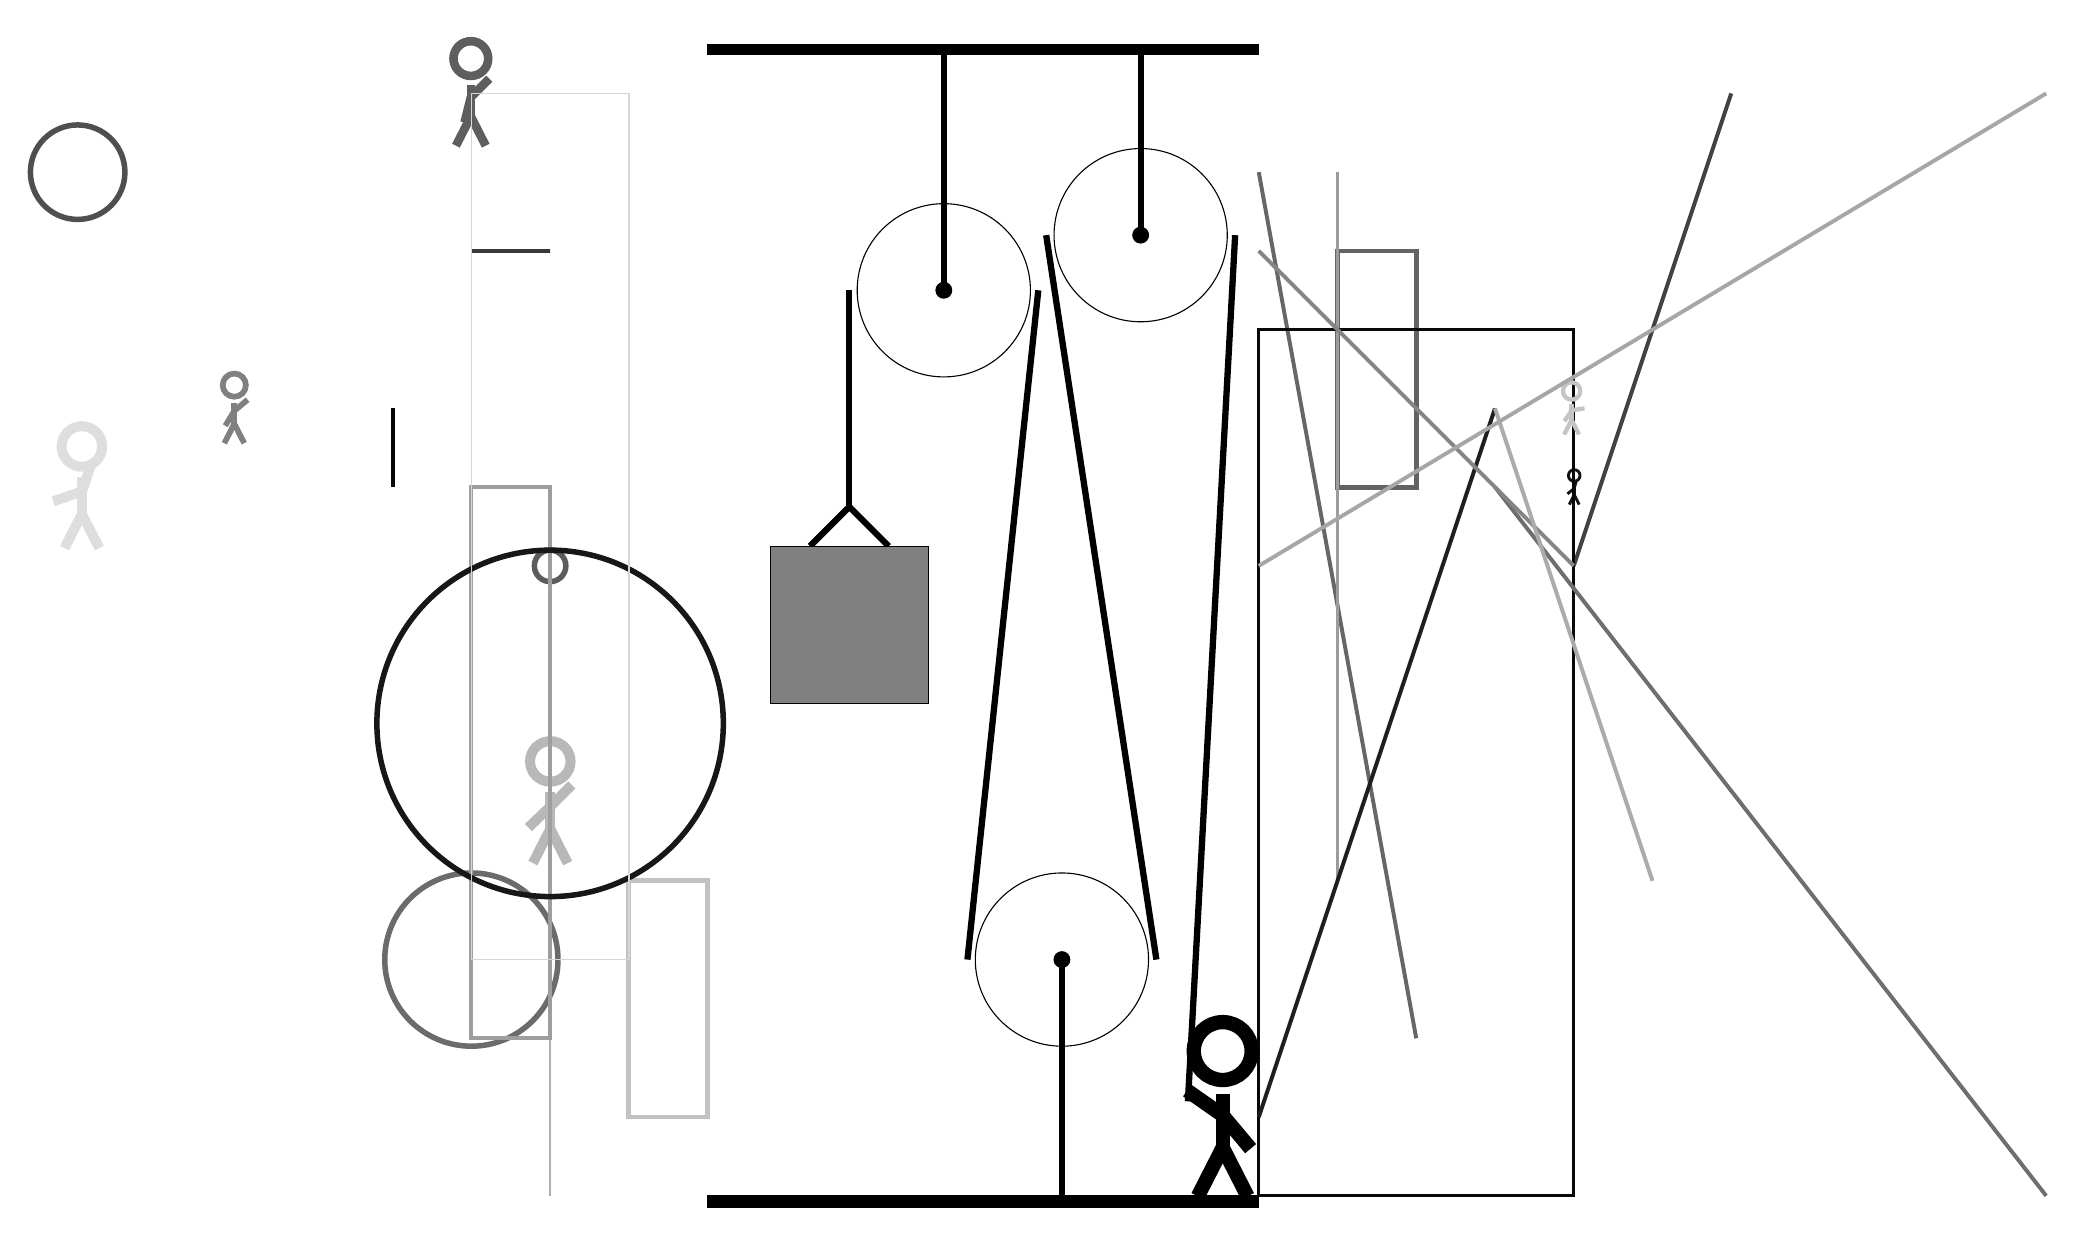
\begin{tikzpicture}
			%%%%% START %%%%%
			
			\draw[fill=black] (-2, 11.5) rectangle (5, 11.625);
			
			\draw[line width=0.6mm, color=black!78] (-4, 9) rectangle (-5, 9);
			
			\draw[line width=0.5mm, color=black!60](5, 10) -- (7, -1);
			\draw[line width=0.6mm, color=black!61] (6, 9) rectangle (7, 6);
			\draw [line width=0.7mm, color=black!64](-4, 5) circle (0.2);
			
			\draw[line width=0.4mm, color=black!39] (6, 10) rectangle (6, 1);
			\draw[line width=0.5mm, color=black!74](9, 5) -- (11, 11);
			\node[line width=0.5mm, color=black!50] at (-8, 7) {\Strichmaxerl[4][59][40]};
			\draw [line width=0.7mm, color=black!58](-5, 0) circle (1.1);
			\draw [line width=0.7mm, color=black!69](-10, 10) circle (0.6);
			\node[line width=0.2mm, color=black!63] at (-5, 11) {\Strichmaxerl[6][76][45]};
			
			\node[line width=0.5mm, color=black!93] at (9, 6) {\Strichmaxerl[2][39][74]};
			\draw[line width=0.4mm, color=black!97] (5, 8) rectangle (9, -3);
			\draw[line width=0.2mm, color=black!31] (-4, 0) rectangle (-4, -3);
			\draw[line width=0.5mm, color=black!57](8, 6) -- (15, -3);
			\node[line width=0.4mm, color=black!28] at (-4, 2) {\Strichmaxerl[7][44][45]};
			\node[line width=0.7mm, color=black!23] at (9, 7) {\Strichmaxerl[3][57][8]};
			\draw[line width=0.5mm, color=black!38] (-4, -1) rectangle (-5, 6);
			
			\draw[line width=0.6mm, color=black!24] (-3, 1) rectangle (-2, -2);
			\draw[line width=0.5mm, color=black!88](8, 7) -- (5, -2);
			
			\draw[line width=0.5mm, color=black!48](9, 5) -- (5, 9);
			\draw [line width=0.7mm, color=black!91](-4, 3) circle (2.2);
			
			\draw[line width=0.5mm, color=black!98](-6, 6) -- (-6, 7);
			\draw[line width=0.2mm, color=black!16] (-3, 0) rectangle (-5, 11);
			\draw[line width=0.5mm, color=black!33](8, 7) -- (10, 1);
			\node[line width=0.3mm, color=black!13] at (-10, 6) {\Strichmaxerl[7][19][71]};
			
			\draw[line width=0.5mm, color=black!35](5, 5) -- (15, 11);
			
			
			\draw (1, 8.5) circle (1.1);
			\draw[fill=black] (1, 8.5) circle (0.1);
			\draw[line width=0.8mm]  (1, 11.5) -- (1, 8.5);
			
			\draw[fill=white](2.5, 0.0) circle (1.1);
			\draw[fill=black] (2.5, 0.0) circle (0.1);
			\draw[line width=0.8mm]  (2.5, -3) -- (2.5, 0.0);
			
			\draw[fill=white](3.5, 9.2) circle (1.1);
			\draw[fill=black] (3.5, 9.2) circle (0.1);
			\draw[line width=0.8mm] (3.5, 11.5) -- (3.5, 9.2);
			
			\draw[line width=0.8mm] (-0.7, 5.25) -- (-0.2, 5.75) -- (0.3, 5.25);
			\draw[fill=black!50] (-1.2, 5.25) rectangle (0.8, 3.25);
			
			\draw[line width=0.8mm] (-0.2, 8.5) -- (-0.2, 5.75);
			\centerarc[line width=0.8mm](1, 8.5)(0:180:1.2000000000000002);
			\draw[line width=0.8mm](2.2, 8.5) -- (1.3, 0.0);
			\centerarc[line width=0.8mm](2.5, 0.0)(180:360:1.2000000000000002);
			\draw[line width=0.8mm](3.7, 0.0) -- (2.3, 9.2);
			\centerarc[line width=0.8mm](3.5, 9.2)(0:180:1.2000000000000002);
			\draw[line width=0.8mm](4.7, 9.2) -- (4.1, -1.8);
			
			\node at (4.5, -1.9) {\Strichmaxerl[10][-35][-50]};
			
			\draw[fill=black] (-2, -3) rectangle (5, -3.15);
			
			%%%%% END %%%%%
		\end{tikzpicture}
	\end{figure}	
\end{document}